% begin module inverse-function-ex5
\begin{frame}
\begin{example}%[Example 5, p. 388]
\begin{columns}[c]
\column{.5\textwidth}
\psset{xunit=0.5cm, yunit=0.5cm}
\begin{pspicture}(-5, -5)(5,5) 
\psframe*[linecolor=white](-5,-5)(5,5) \tiny
\psaxes[ticks=none, labels=none]{<->}(0,0)(-4.55,-5)(4.5,5)
\psline(1, -0.1)(1, 0.1)
\rput[t](1, -0.2){\tiny$1$}
\psline(-1, -0.1)(-1, 0.1)
\psline(-0.1, 1)(0.1, 1)
\rput[br](-0.2, 1){\tiny$1$}
\psline(-0.1, -1)(0.1, -1)
\uncover<3>{
%Function formula: sqrt{}(- (x)) 
\psplot[linecolor=red, plotpoints=1000]{-4.5}{0}{x -1 mul sqrt }
\rput(-2, 2.2){\tiny$y=\sqrt{-x}$}
}
\uncover<4->{
%Function formula: sqrt{}(- (x)) 
\psplot[linecolor=gray, plotpoints=1000]{-4.5}{0}{x -1 mul sqrt }
\rput(-2, 2.2){\color{gray}\tiny$y=\sqrt{-x}$}
}
\uncover<2>{
 %Function formula: sqrt{}(x) 
\psplot[linecolor=red, plotpoints=1000]{0}{4.5}{x sqrt } 
\rput(2.4, 1){\tiny $y=\sqrt{x}$}
}
\uncover<3->{
 %Function formula: sqrt{}(x) 
\psplot[linecolor=gray, plotpoints=1000]{0}{4.5}{x sqrt } 
\rput(2.4, 1){\color{gray}\tiny $y=\sqrt{x}$}
}
\uncover<4>{
%Function formula: sqrt{}(- (x)-1) 
\psplot[linecolor=red, plotpoints=1000]{-4.5}{-1}{-1 x -1 mul add sqrt }
\rput[r](-2.3, 0.55){\tiny$y=f(x)$}
}
\uncover<5->{
%Function formula: sqrt{}(- (x)-1) 
\psplot[linecolor=gray, plotpoints=1000]{-4.5}{-1}{-1 x -1 mul add sqrt }
\rput[r](-2.3, 0.55){\color{gray}\tiny$y=f(x)$}
}

\uncover<5>{
%Function formula: - ((x)^{2})-1 
\psplot[linecolor=red, plotpoints=1000]{0}{2}{-1 x 2 exp -1 mul add } 
\rput[l](1.3, -2){\tiny$y=f^{-1}(x)$}
\psline[linecolor=blue, linestyle=dashed] (-4.5, -4.5)(4.5, 4.5)
\rput[tl](-3, -3.2){\tiny $y=x$}
}
\end{pspicture} 
%\ \only<handout:0| -1>{%
%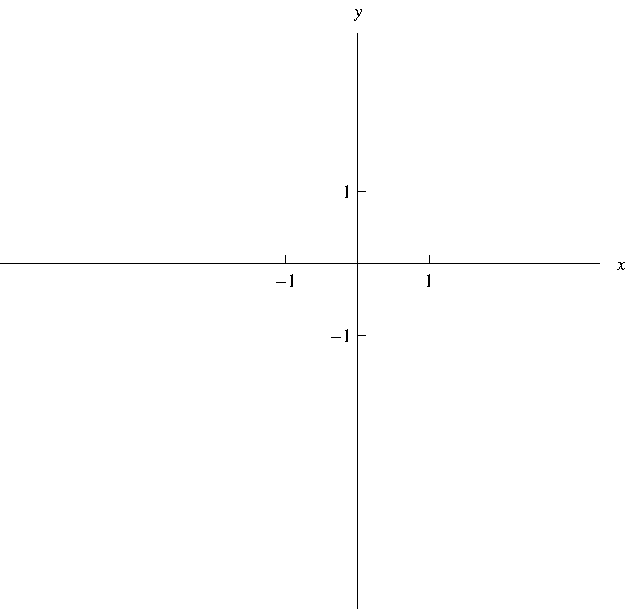
\includegraphics[height=4.5cm]{inverse-functions/pictures/07-01-ex5a.pdf}%
%}%
%\only<handout:0| 2>{%
%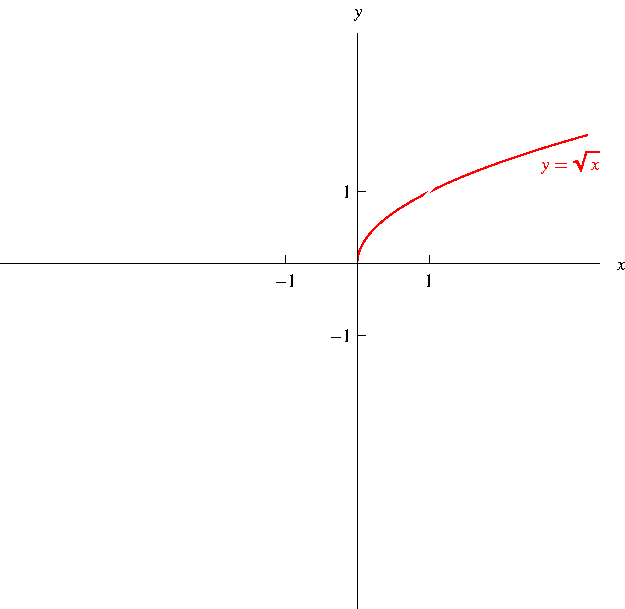
\includegraphics[height=4.5cm]{inverse-functions/pictures/07-01-ex5b.pdf}%
%}%
%\only<handout:0| 3>{%
%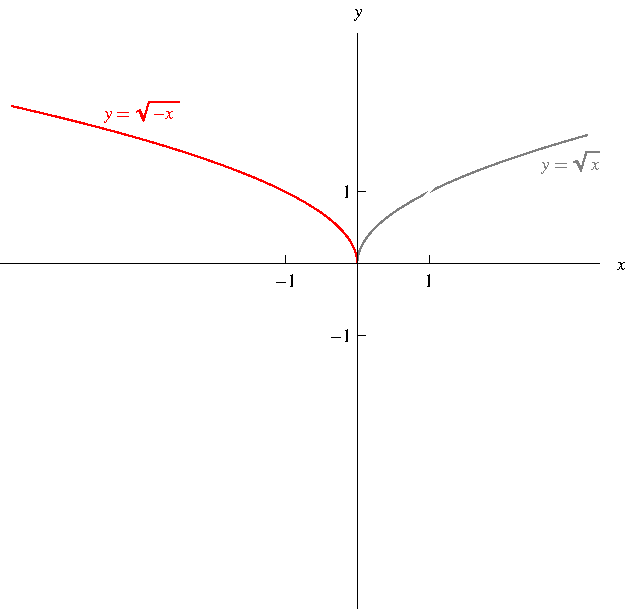
\includegraphics[height=4.5cm]{inverse-functions/pictures/07-01-ex5c.pdf}%
%}%
%\only<handout:0| 4>{%
%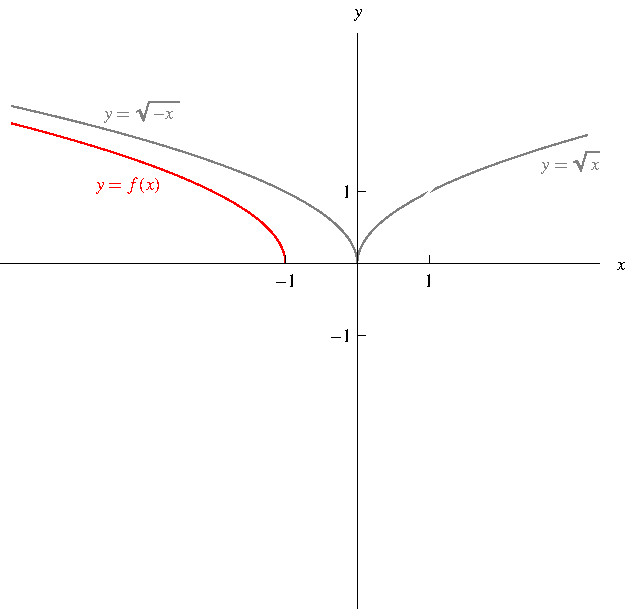
\includegraphics[height=4.5cm]{inverse-functions/pictures/07-01-ex5d.pdf}%
%}%
%\only<handout:1| 5->{%
%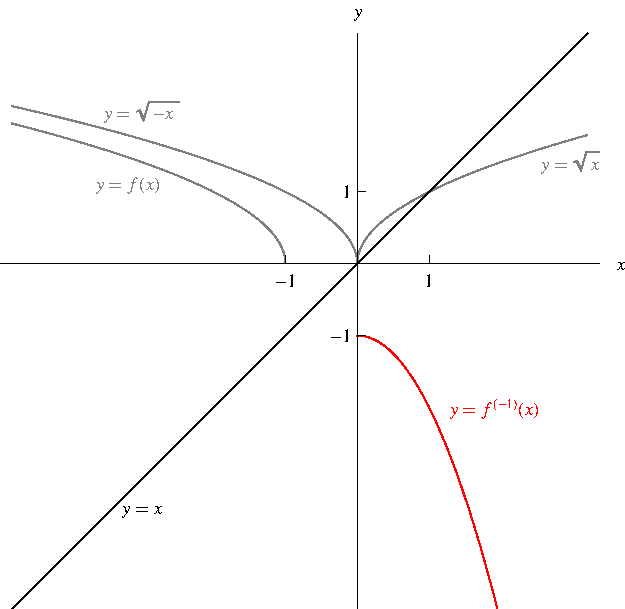
\includegraphics[height=4.5cm]{inverse-functions/pictures/07-01-ex5e.pdf}%
%}%

\column{.5\textwidth}
Sketch the graph of $f(x) = \sqrt{-x - 1}$ and its inverse function.
\end{columns}
\begin{itemize}
\item<2->  First draw the graph of $y = \sqrt{x}$.
\item<3->  $y = \sqrt{-x}$ is the reflection of $y = \sqrt{x}$ in the $y$-axis.
\item<4->  $y = f(x) = \sqrt{-x - 1}$ is the shift of $y = \sqrt{-x}$ one unit to the left.
\item<5->  $y = f^{-1}(x)$ is the reflection of $y = f(x)$ across the line $y = x$.
\end{itemize}
\end{example}
\end{frame}
% end module inverse-function-ex5